% book.tex -- Copyright (c) 2004, Brian C. Ladd
% 
% Author : Brian C. Ladd 
% Created: Wed Jul 07 12:03:49 2004 by blad
% Revised: Fri Dec 28 15:27:43 2007 by blad
% 
\def\FileCreated{Wed Jul 07 12:03:49 2004}
\def\FileRevised{Fri Dec 28 15:27:43 2007}
\documentclass[12pt,oneside]{memoir}
\usepackage{epsfig}
\usepackage{graphicx}
\usepackage[usenames]{color}
\usepackage{xltxtra}
\usepackage{fontspec}
\usepackage{textcomp}
\usepackage{pstricks}
\usepackage{listings}[2000/08/23] 

\usepackage{rotating}
\usepackage{exercise}
\definecolor{nicered}{rgb}{.647,.129,.149}
\definecolor{listinggray}{gray}{0.9}
\definecolor{templategrey}{gray}{0.30}
\definecolor{commandlinebackground}{gray}{0.25}
\definecolor{commandlineforeground}{gray}{0.85}
\definecolor{commandpromptforeground}{gray}{0.55}
% ----- Fonts -----
\defaultfontfeatures{Scale=MatchLowercase,Mapping=tex-text}
\setmainfont{Gentium Book Basic}
\setmonofont{Inconsolata}
\setsansfont{Arial}
% ----- Fonts -----
\newcommand\code[1]{\lstinline^#1^}
\newcommand\fname[1]{\texttt{#1}}

\lstset{language=java,
  basicstyle=\small\ttfamily,
  numbers=none, 
  numberstyle=\tiny, 
  stepnumber=1, 
  numbersep=5pt,
  frame=single,
  captionpos=b,
  rulecolor=\color{nicered}
}

\lstdefinelanguage{cline}
{
  morecomment=[s][\color{commandpromptforeground}]{ }{ },
} 

\lstnewenvironment{commandline}[1][]
{\lstset{language=cline,numbers=none,frame=none,backgroundcolor=\color{commandlinebackground},basicstyle=\color{commandlineforeground},nolol,#1}}
{}

\newenvironment{Checkpoint}[1]{%
  \begin{Exercise}[name={Checkpoint},title={#1}]}{%
  \end{Exercise}%
  \textbf{Show your work on Checkpoint~\theExercise{} to the lab monitor, %
    answering any necessary questions for them.  Have them sign before continuing.}}

\newcommand{\artDir}{../art}
\newcommand{\lab}[2]{%
  \title{CIS 201 Computer Science I\\Fall 2009 Lab #1\\#2}%
  \maketitle%
}

\setlength{\hoffset}{0in}
\setlength{\voffset}{0in}
\settypeblocksize{9.5in}{7.5in}{*}
\setlrmargins{0.5in}{*}{1}
\setulmargins{0.75in}{*}{*}
\setheadfoot{\onelineskip}{2\onelineskip}
\checkandfixthelayout

\begin{document}

\lab{08}{Tic Tac Toe}

\begin{itemize}
\item Implementing a class revisited
\item Using \code{ArrayList}
\item Game components with ``state''
\item Restarting a game
\end{itemize}

\begin{figure}[htb]
  \begin{center}    
    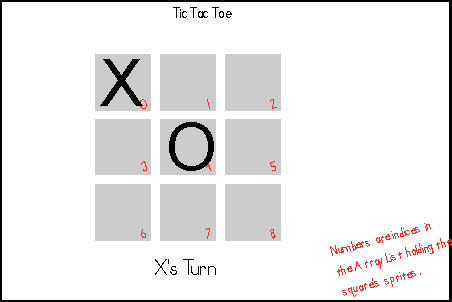
\includegraphics[width=5in]{\artDir/ticTacToe-design}  
    \caption{TicTacToe Design}
    \label{fig:design}
  \end{center}
\end{figure}

\begin{Checkpoint}{Getting Started}

  Consider a simple version of Tic Tac Toe: your \code{Game} creates
  and positions nine sprites on the screen. Then, in \code{advance}
  you would check for mouse clicks, comparing any click to each of the
  sprites. If one is clicked \emph{and} it is empty, update the sprite
  with the current player's symbol and change who's turn it is. Make
  sure to check for winning and draws somewhere.

  Think about how \code{advance} would look. Assuming the sprites are
  in an \code{ArrayList}, there would be a big loop with many nested
  \code{if} statements in it. This code is too complex to hold in your
  mind, all at once.

  How do computer programmers respond to complexity?

  \emph{Abstraction!} (Hopefully you got that one.)

  Abstraction is the hiding of details of some rule or some
  component. It can be applied by writing methods with descriptive
  names that make it easier to express the solution at a higher
  level. Abstraction can also be applied by breaking responsibility
  for the solution across multiple components. 

  The ``simple'' approach given above is difficult because the Tic Tac
  Toe game is responsible for handling both game-level details
  \emph{and} square-level details. A separation of responsibility is
  possible if we build ``smart'' squares; this is a standard technique
  in object-oriented design, the creation of objects that ``know what
  to do''.

  Before reading on, you and your partner should pull out a piece of
  paper and write down what activities a Tic Tac Toe game must
  support. Divide up your list into game-level and move-level
  activities.

  Show your list of activities to one of the lab instructors; document
  your list by including it in a header comment for the \code{Game}
  extending class.
\end{Checkpoint}

\newpage
\begin{Checkpoint}{Define classes}
  When designing this lab, the following responsibilities seemed
  necessary.  Each square is responsible for:
  \begin{itemize}
  \item Advancing the state of the square (each frame):
    \begin{itemize}
    \item Checking whether it is legal to click on the square (it is
      not legal if the square is not empty)
    \item Checking whether it has been clicked
    \item If it has been clicked, updating according to which player's
      turn it was and ending the turn.
    \end{itemize}
  \item \code{isEmpty} to determine whether or not the square is
    occupied.
  \item Return the current state of the square (``X'', ``O'', or ``'').
  \end{itemize}

  The game is then responsible for
  \begin{itemize}
  \item Setting up the game: creating the squares, scaling and
    positioning them.
  \item Advancing every square every frame.
  \item Showing status.
  \item Returning the current player (``X'', ``O'').
  \item Ending a turn.
    \begin{itemize}
    \item Checking if the current player has won.
    \item Checking if there is a cat's game.
    \item Otherwise, change which player's turn it is.
    \end{itemize}
  \end{itemize}

  This lab builds two cooperating classes, \code{TicTacToe} and
  \code{TicTacToeSquare}, each fulfilling one of these sets of
  requirements.

  Note \emph{how} the two classes cooperate: \code{TicTacToe} 
  needs references to all of the squares so that it can call
  \code{advance} for each of them; \code{TicTacToeSquare} needs a
  reference to the game of which it is a part to be able to check for
  mouse clicks, determine whose turn it is, and to be able to end a
  turn. While \code{Game.getCurrentGame()}  suffices for mouse clicks,
  the other actions are \code{TicTacToe} specific: each square is
  constructed with a reference to the game of which it is a part.

  Start the \code{TicTacToe} and \code{TicTacToeSquare} classes in a
  Lab 8 directory. 

  One should extend \code{Game}, the other \code{CompositeSprite}. As
  discussed in class, build this lab one piece at a time; that means
  first get the squares to draw in the right places. Then make them
  aware of mouse clicks, and then, finally, we will make the game
  check for end-of-game conditions.

  \code{TicTacToeSquare} should create a rectangle sprite of a dark
  (non-black) color. The ``X''/``O'' sprite comes later. This means
  writing a \emph{constructor} for the class; there is no need for
  anything else right now.

  What \emph{parameters} does the constructor require? Since a
  \code{TicTacToe} is required for determining  whose turn it is and
  ending a turn, there needs to be a field in \code{TicTacToeSquare}
  referring to a \code{TicTacToe} game. How would you declare a
  \emph{field} of type \code{TicTacToe}? Declare such a field in
  \code{TicTacToeSquare}.

  If the constructor takes a \code{TicTacToe} reference, how is it
  called when constructing a new square? Remember \code{this}? In any
  method in \code{TicTacToe}, \code{this} is a reference to a
  \code{TicTacToe} object. The call (probably in \code{setup}) in
  \code{TicTacToe} looks something like this:

  \begin{lstlisting}
    TicTacToeSquare someSquare = new TicTacToeSquare(this);
  \end{lstlisting}

  The reference to the \code{TicTacToe} makes it possible to check who's
  turn it is and get mouse clicks.

  \code{TicTacToe} should construct nine \code{TicTacToeSquare}
  objects and put them in an \code{ArrayList}. They should be
  distributed in a 3 x 3 grid against the top of the screen. Each
  should be 0.20 screens square, centers of rows and columns should be
  0.25 apart (at 0.25, 0.50, and 0.75 for the columns, at 0.10, 0.35,
  and 0.60 for the rows).

  How the heck should we go from an index into an \code{ArrayList} to
  its corresponding screen coordinates? You should create two methods
  for \code{TicTacToe}, \code{row} and \code{column}, each of which
  takes a single integer parameter, the index into the
  \code{ArrayList} and then returns the row (or column) where that
  element belongs (0, 1, or 2). Then use a simple linear
  equation to go from column number to screen coordinates (and the
  same for rows).

  \begin{lstlisting}
   /**
    * Convert the index, range [0-9), into the corresponding row 
    * on the screen, range [0-2).
    */
    public int row(int index) {
      // ... your code here ...
    }

   /**
    * Convert the index, range [0-9), into the corresponding column
    * on the screen, range [0-2).
    */
    public int column(int index) {
      // ... your code here ...
    }
  \end{lstlisting}

  You should also set up an integer to keep track of which player's
  turn it is (0 for ``X'', 1 for ``O''), a \code{StringSprite} to hold
  a status message (scale to 0.10, position at the bottom-center of
  screen at 0.9 down (the reason the board is so high)).

  Explain your \code{row} and \code{column} methods to the lab
  instructor.
\end{Checkpoint}

\begin{Checkpoint}{Update status.}
  Create a method, \code{updateStatus}, which takes a \code{String}
  and updates the message displayed in the status string. Modify
  \code{setup} so that the status line displays which player's turn it
  is using your new method.
\end{Checkpoint}

\begin{Checkpoint}{Square state}
  As documented above, a square must track its contents; this means a
  \code{content} field. The type should probably be an integer (to
  match the turn tracker in the game to ease picking what symbol to
  put in the square). Initialize content to a third value (not the one
  for ``X'' or ``O'') to indicate empty; perhaps -1.

  Implement both a setter and a getter for the \code{content}
  field. 

  In the setter, you need to update a display value. Add a
  \code{StringSprite} to \code{TicTacToeSquare}. The scale should be
  1.0 and it should initially (in the constructor) hold the empty
  string. It should use some non-FANG Blue light color. When setting
  the content of the square, set the text to ``X'' if the content is
  set to the x content value or ``O'' if the content is set to the o
  content value.

  Implement \code{isEmpty} (a public, Boolean method) which returns
  \code{true} if the square is empty, \code{false} otherwise.
\end{Checkpoint}


\begin{Checkpoint}{Square advance}
  Declare a new method for \code{TicTacToeSquare} called \code{advance};
  model it on the \code{advance} in the game. Inside the method do the
  following:

  \begin{lstlisting}
    if ((this square is empty) && (the mouse has been clicked)) 
      if (this sprite intersects mouse click)
        update content
        update appearance of StringSprite
        call theGame.finishTurn
  \end{lstlisting}

  In \code{TicTacToe}, call the \code{advance} method for every square
  on every frame. If you have to do something with every element in an
  \code{ArrayList}, \emph{what should you be thinking}?

  You can comment out the call to \code{finishTurn}; that should permit
  you to compile your program and click on the various squares and make
  them all ``X'' (turn doesn't change yet). Remember, incremental
  development, getting a little bit working before moving on, is another
  way to control complexity.  
\end{Checkpoint}

\begin{Checkpoint}{Finish turn}
  Implement \code{TicTacToe.finishTurn}: it takes no
  parameters and just changes who's turn it is. If turn was 0, make it 1
  and if it was 1, make it 0.

  Uncomment the call to \code{finishTurn} in the \code{advance} method
  of \code{TicTacToeSquare}.  
\end{Checkpoint}

\begin{Checkpoint}{Winning and losing}
  Add checking for winning board position and cat's
  game. You should modify \code{finishTurn} to something like the
  following:

  \begin{lstlisting}
    if (winner(turn)) {
      // handle win
    } else if (catsGame()) {
      // handle cat's 
    } else {
      // change who's turn it is as before
    }
  \end{lstlisting}

  Now you have to write the two methods listed. How will you check if it
  is a cat's game? Given that squares can give you their content it
  should be easy to check whether or not there are any empty squares:
  call \code{isEmpty} in \code{catsGame} for every square in the
  game...every square in the \code{ArrayList}...\emph{what should you be
  thinking}? 

  The \code{winner} method is a touch messier: check the eight different
  ways that a game can be won. The player who just moved is provided as
  a parameter to the method so you can just check for contents matching
  that value.

  To make the logic easier to follow, use a method, say \code{ndx}
  which, given a row and a column, returns the index in the
  \code{ArrayList} corresponding to that element. That means that
  checking one of the diagonals would just be:

  \begin{lstlisting}
    (board.get(ndx(0, 0)).getContent() == turn &&
    board.get(ndx(1, 1)).getContent() == turn &&
    board.get(ndx(2, 2)).getContent() == turn)
  \end{lstlisting}

  This Boolean expression will be true if and only if the values on the
  main diagonal equal the turn variable. So long as \code{turn} is
  either 0 or 1, we will only return true for a win along that diagonal.
\end{Checkpoint}

\begin{Checkpoint}{New game}
  Is starting over a \emph{square}-level responsibility or a
  \emph{game}-level responsibility? 

  In the correct class define a \code{boolean} field,
  \code{waiting}. When \code{waiting} is \code{true}, the game is
  waiting to start over. In \code{advance}, rather than checking for
  mouse clicks on squares, check for the user pressing the space
  bar. If they do, call \code{startOver()} to restart the game
  (\code{setup} is called again).

  The \code{waiting} flag is cleared (set to \code{false}) in
  \code{setup}. Where is it set \code{true}? Consider the three-way
  \code{if} statement where you check for winning or cat's games. If
  the game is over (win or cat's), set the flag and update the status
  message. Whenever a game ends, \code{waiting} is set and when a game
  starts it is cleared.
\end{Checkpoint}

Also make sure that both partners have copies of the program. This
program has some bearing on upcoming assignments; you'll want this
code around. Comments will also be very helpful in this program for
exactly that reason.

\Large{Log off of the lab computer you are using before leaving they
  lab. Anyone entering the lab has unlimited access to your files if
  you remain logged on. \textbf{DO NOT} turn off lab computers! They
  are a shared resource and there might be someone else logged in to
  ``your'' machine.}
\end{document}

%%% Local Variables: 
%%% mode: latex
%%% End: 

% LocalWords:  Moodle Ladd's login emacs
